\section{Dagster}
De derde tool waarvan een Proof of Concept gemaakt wordt is Dagster. Dit zal, in combinatie met MLFlow, gebruikt worden voor het lokaal uitvoeren van Machine Learning pipelines. Hierbij worden alle aanpassingen in de code van het framework vergeleken met de originele code van opdracht 3 van het opleidingsonderdeel Machine Learning Operations.
\subsection{Installatie}
De installatie van Dagster verloopt via de package manager \texttt{pip}. Dagster ondersteunt Python versies 3.8 tot 3.12 en kan met het volgende commando worden geïnstalleerd:
\begin{minted}[frame=lines,breaklines,linenos]{bash}
    pip install dagster dagster-webserver
\end{minted}
Om Dagster te installeren op een Mac met een Apple Silicon chip moet het volgende commando gebruikt worden:
\begin{minted}[frame=lines,breaklines,linenos]{bash}
    pip install dagster dagster-webserver --find-links=https://github.com/dagster-io/build-grpcio/wiki/Wheels
\end{minted}
Na het installeren van Dagster kan er een project aangemaakt worden via de terminal met het volgende commando:
\begin{minted}[frame=lines,breaklines,linenos]{bash}
    dagster project scaffold --name my-dagster-project
\end{minted}
Het bovenstaande commando maakt een mapstructuur aan met ruimte voor de pipeline en andere bestanden voor het opzetten van een project in Dagster. Er is ook een parameter \textit{name} die de naam van het project definieert.
Na het aanmaken van het project kan de webserver worden opgestart. Dit kan met het volgende commando. Voordat je het commando uitvoert, moet je echter naar de map navigeren waar het Dagster-project zich bevindt:
\begin{minted}[frame=lines,breaklines,linenos]{bash}
    dagster dev
\end{minted}
\subsection{Dashboard}
Na het opstarten van de webserver kun je via het webadres in de terminal naar het Dagster-dashboard gaan. Het Dagster-dashboard is een omgeving waarin alle pipelines worden beheerd.
Het dashboard ziet eruit zoals in figuur~\ref{fig:Dagser_assets}
\begin{figure}[h]
    \centering
    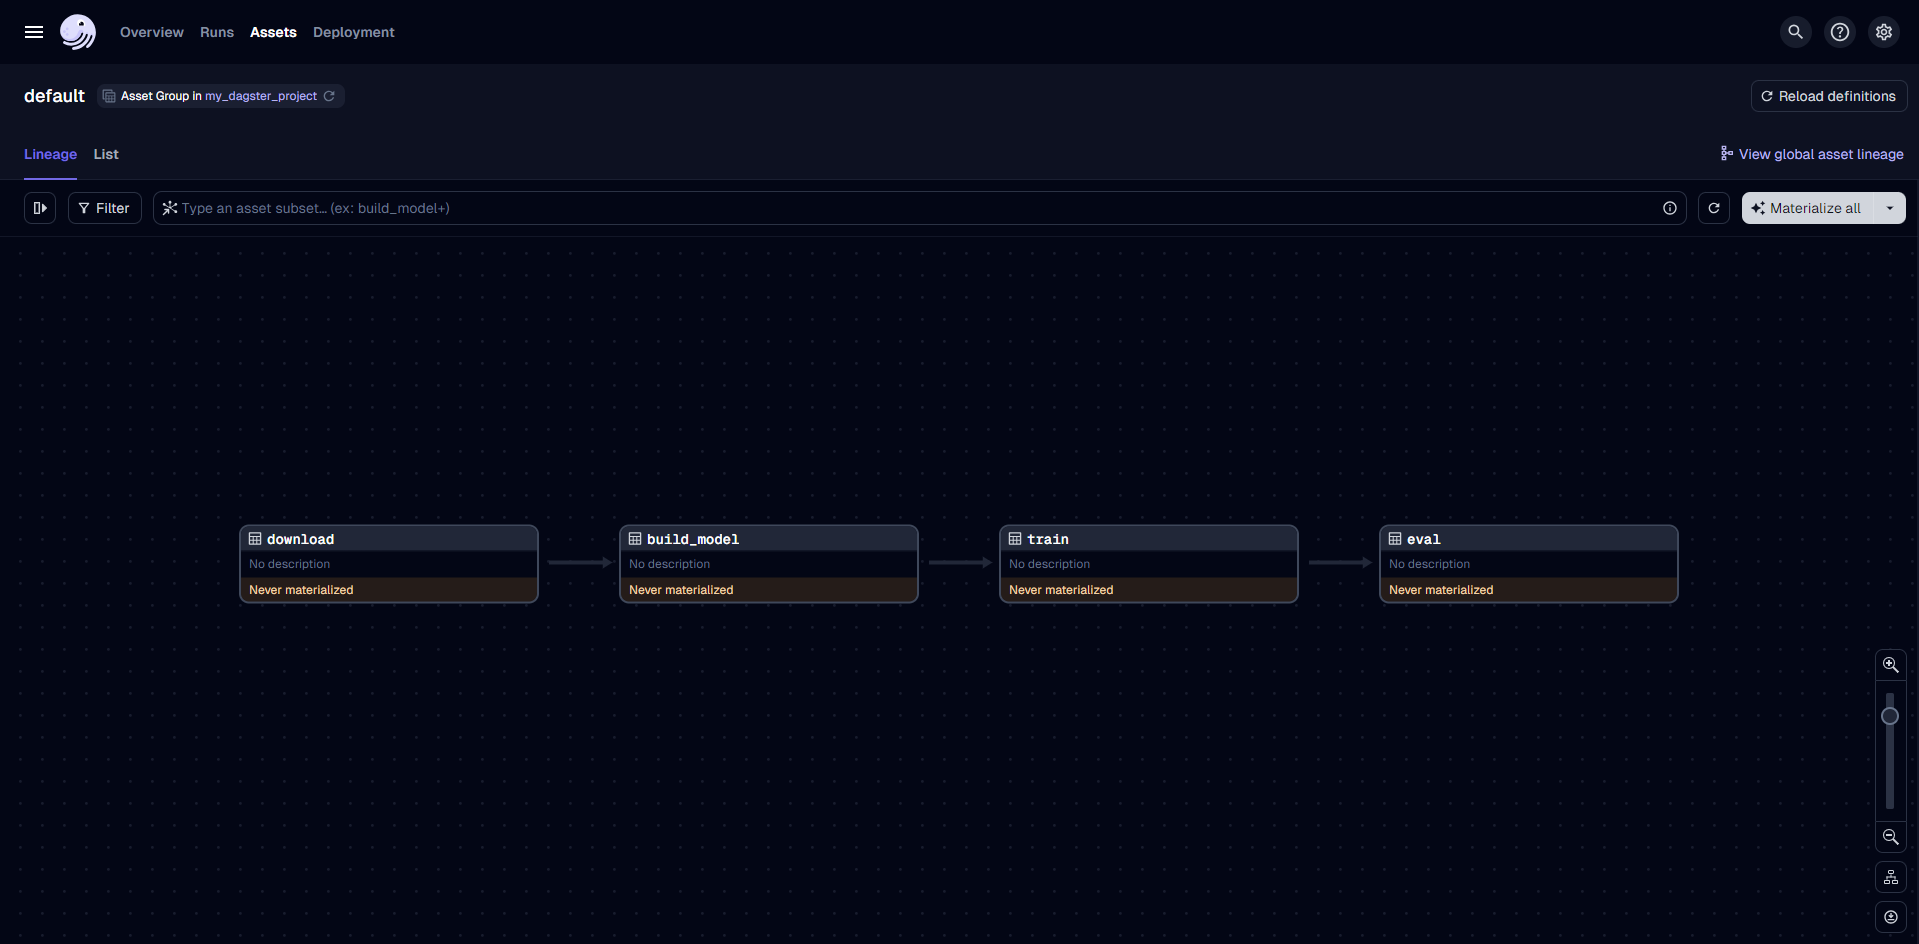
\includegraphics[width=0.9\linewidth]{graphics/Dagster_Assets.PNG}
    \caption{Dagster assets overview}
    \label{fig:Dagser_assets}
\end{figure}
Standaard word je naar de asset-pagina van Dagster verwezen wanneer je op de link in de terminal klikt, zoals weergegeven in figuur~\ref{fig:Dagser_assets}.
De functies die kunnen worden gezien op Figuur~\ref{fig:Dagser_assets} zijn:

\begin{itemize}
    \item \textbf{Overview:} Geeft een tijdlijn van alle uitgevoerde pipelines weer.
    \item \textbf{Runs:} Geeft een overzicht van alle uitgevoerde pipelines weer.
    \item \textbf{Assets:} Geeft alle \textit{assets} weer van de huidige Machine Learning pipeline.
    \item \textbf{Deployments:} Geeft alle deployments weer. Dit zijn alle projecten in de huidige map.
\end{itemize}

De \textit{runs} pagina ziet er uit zoals in figuur~\ref{fig:Dagser_runs}
\begin{figure}[h]
    \centering
    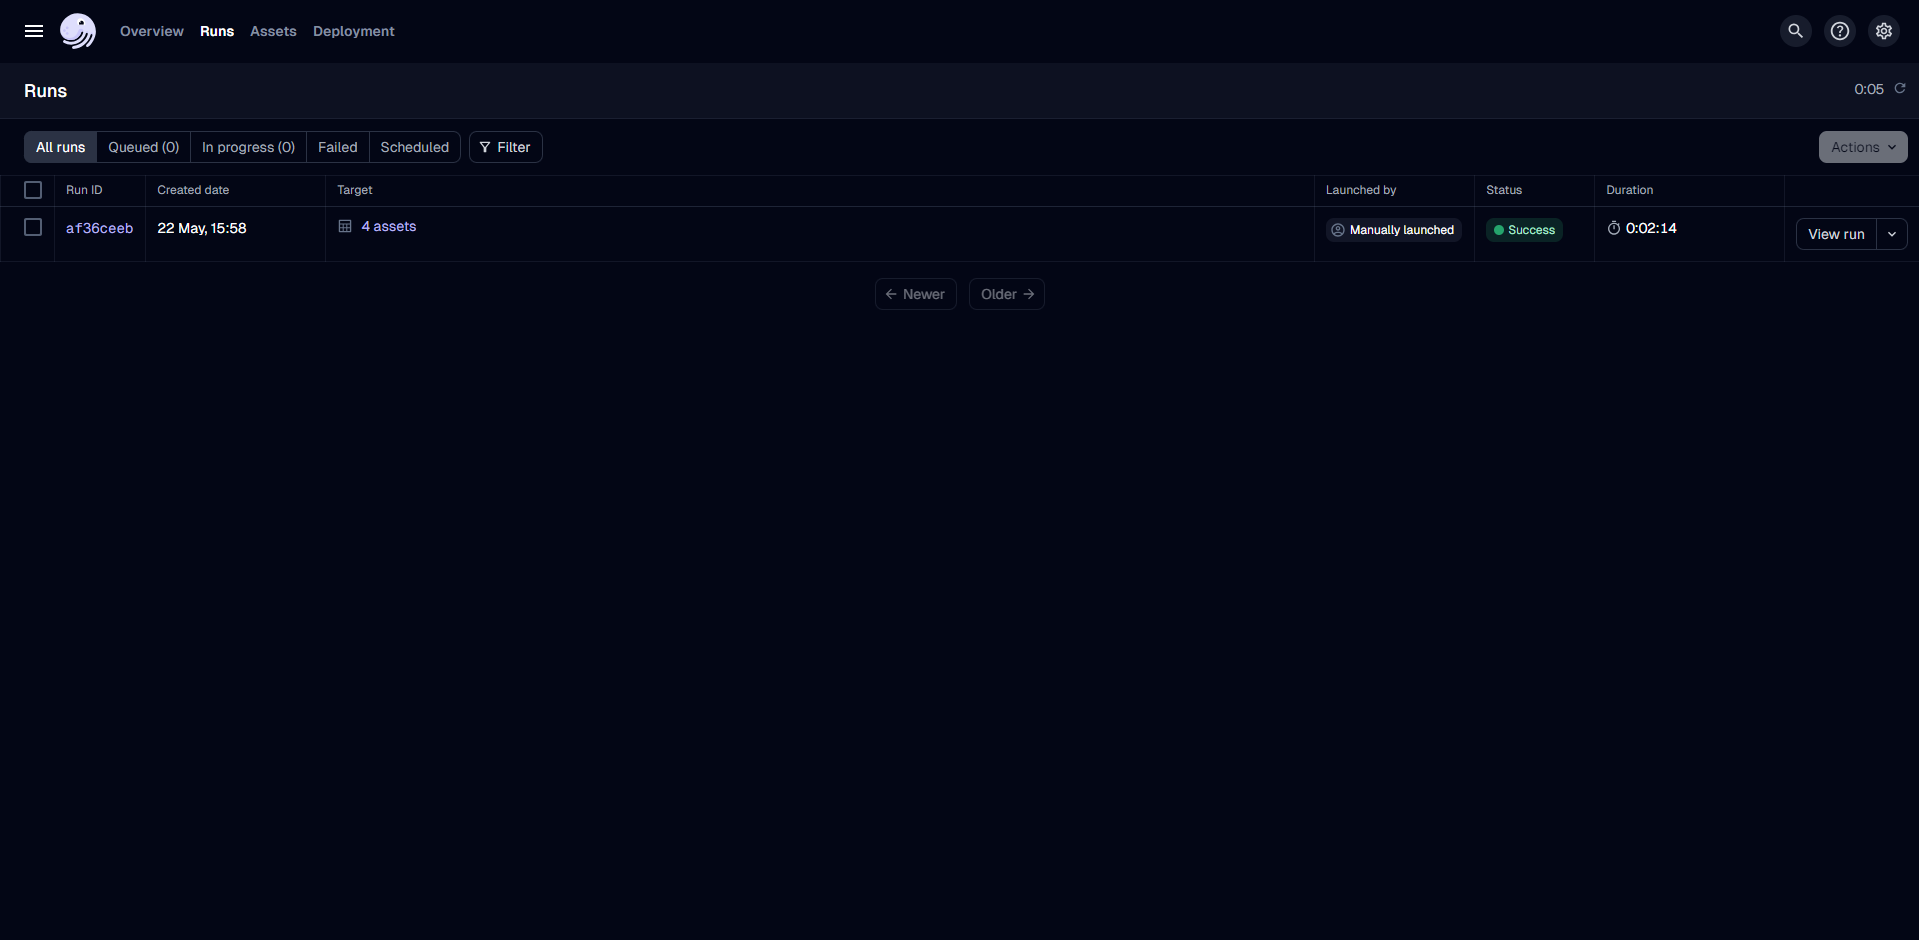
\includegraphics[width=0.9\linewidth]{graphics/Dagster_Runs.PNG}
    \caption{Dagster runs overview}
    \label{fig:Dagser_runs}
\end{figure}

Bij het overzicht van de uitvoeringen van de pipelines kan een pipeline geselecteerd worden om meer details te zien. Figuur~\ref{fig:Dagser_details} toont hoe deze pagina eruit ziet.
\begin{figure}[h]
    \centering
    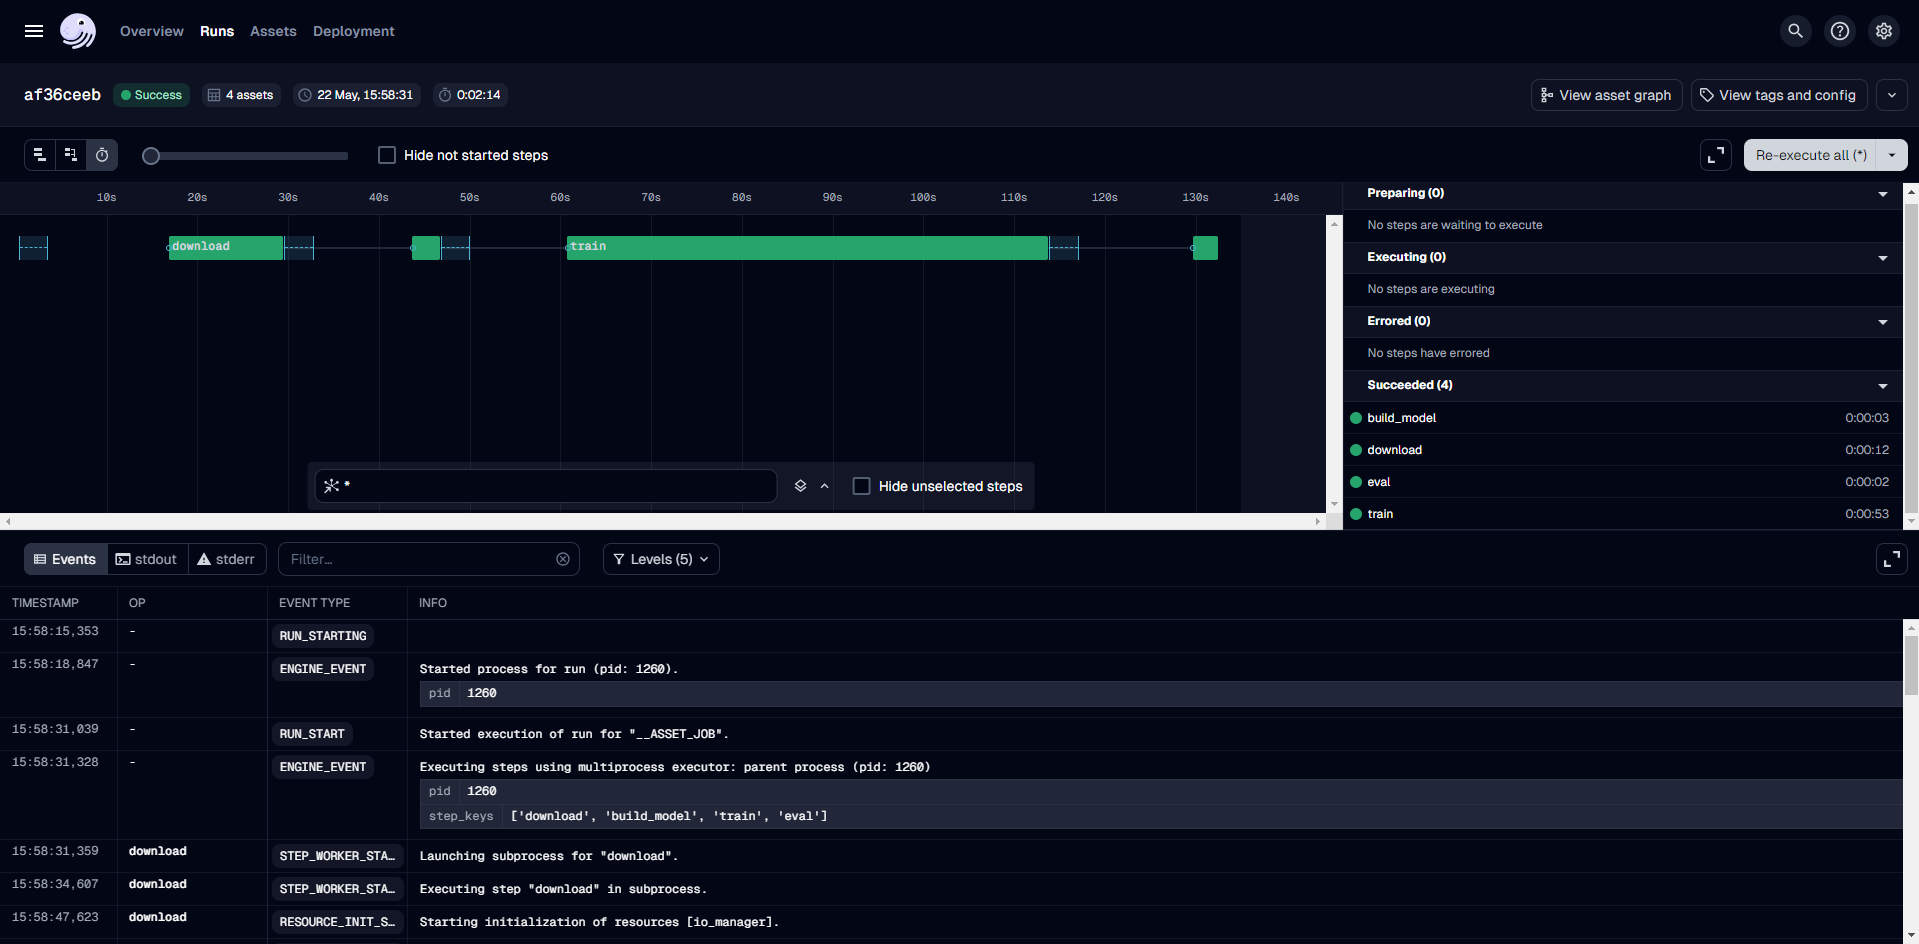
\includegraphics[width=0.9\linewidth]{graphics/Dagster_Flow.PNG}
    \caption{Dagster pipeline detauks}
    \label{fig:Dagser_details}
\end{figure}
\subsection{Uitvoering}
Origineel bevatte het preprocessingsgedeelte zowel het downloaden als het verwerken van de afbeeldingen. Voor gebruik in Dagster is dit echter opgesplitst in twee aparte stappen: het downloaden en het verwerken van de afbeeldingen gebeurt nu afzonderlijk. Ook bij het maken van het model wordt het model eerst gebouwd en pas daarna getraind. In de originele code gebeurde dit in één functie.
De volledige code van de pipeline is te vinden in de GitHub-repository\footnote{\url{https://github.com/casperaudenaert/BP/tree/main/PoC/Dagster}}van deze Proof of Concept.
Alle functies worden \textit{assets} in Dagster. Hierdoor kan de webserver deze herkennen en weergeven op het dashboard. Er is geen speciale functie of decorator nodig om een pipeline in de code te maken.
\subsection{Pipeline}
In vergelijking met andere frameworks heeft Dagster geen speciale functie of decorator voor het maken van een pipeline. De volgorde wordt bepaald door de parameter \textit{deps} mee te geven aan de \textit{asset}.
Een voorbeeld van hoe dat een asset eruit ziet bij Dagster:
\begin{minted}[frame=lines,breaklines,linenos]{python}
    @asset(deps=[train])
    def eval():
        model = keras.models.load_model('my_model.h5')
        test_datagen = ImageDataGenerator(rescale=1.0 / 255.0)

        test_generator = test_datagen.flow_from_directory(
            f"{DATASET}/test",
            target_size=IMAGE_SIZE,
            batch_size=BATCH_SIZE,
            class_mode='binary',
        )
        mlflow.keras.autolog(log_models=False, log_model_signatures=False)
        test_loss, test_accuracy = model.evaluate(
            test_generator,
            steps=len(test_generator)
        )
        print('Test accuracy:', test_accuracy)
        print('Test Loss:', test_loss)
\end{minted}
De bovenstaande code is bedoeld voor het evalueren van een model met behulp van Dagster. De \textit{asset} decorator zorgt ervoor dat de lokale omgeving de functie kan vinden, en de parameter \textit{deps} geeft aan dat de evaluatiefunctie na het trainen van het model moet worden uitgevoerd.
\subsection{Problemen}
Het probleem bij Dagster was dat verschillende datatypes niet ondersteund werden als parameters voor \textit{assets}, waardoor het model niet kon worden doorgegeven aan de volgende functie. Om dit op te lossen, is het model lokaal opgeslagen en in de opeenvolgende functies opnieuw ingelezen. Dit proces wordt herhaald voor elke opeenvolgende functie.
\subsection{Cloud}
Voor het verbinden met de cloud zijn er twee opties:
\begin{itemize}
    \item \textbf{Codevoorbeeld\footnote{\url{https://dagster.io/templates}}:} Dagster biedt voorbeeldprojecten met verschillende integraties. Dit zijn GitHub-repositories die gedownload kunnen worden om zelf gebruik te maken van de integraties.
    \item \textbf{Documentatie\footnote{\url{https://docs.dagster.io/integrations}}:} Dagster heeft een pagina waarop alle integraties worden gelijst en hoe deze gebruikt moeten worden. Dit gebeurt meestal aan de hand van een \textit{pip}-pakket, waarbij ook een voorbeeld staat van hoe je het pakket moet gebruiken.
\end{itemize}

Voor het overzetten van lokaal naar de cloud is het dus een keuze tussen zelf integreren met de documentatie of beginnen met een startvoorbeeld dat Dagster aanbiedt op hun GitHub-repository.